%        File: memoria.tex
%     Created: sáb jun 28 01:00  2008 C
% Last Change: sáb jun 28 01:00  2008 C
%
\documentclass[a4paper,spanish,12pt]{book}
\title{BLAS: Base Layer for Application Services}
\author{Eduardo Orive Vinuesa}
\usepackage{babel}
\usepackage{times}
\usepackage[T1]{fontenc}
\usepackage[utf8]{inputenc}
\usepackage[left=2.5cm, right=2.5cm]{geometry}
\usepackage{a4}
\usepackage{makeidx}
\usepackage{graphicx}
\usepackage{float}
\usepackage{url}
\usepackage{setspace}
\onehalfspacing
\usepackage{fancyheadings}
\usepackage{wrapfig}

\begin{document}
\tableofcontents

\maketitle
%cuerpo del documento

\chapter{Introducción}
Actualmente casi la totalidad de las instalaciones inform\'aticas son redes, y una mayoria de estas est\'an conectadas a Internet o incluso la propia Internet forma parte de estas.

\section{Historia de los servicios informáticos}
Despu\'es del desarrollo de la primera generación de computadoras el número de estas empezo a aumentar, aunque su disponibilidad estaba normalmente limitada a una unidad por cada entidad (instituciones educativas e instalaciones militares). Estas máquinas requerían de un entorno ambiental muy concreto y el acceso instalaciones donde se albergaban estaba severamente restringido. Por estas mismas limitaciones y para maximizar la disponibilidad se ideó un sistema limitado de terminales remotas, los teletipos, cuya funcion era comunicar con el ordenador central pudiendo utilizar enlaces dedicados o conmutados (lineas telefónicas), permitir la inserción de programas y recuperar el resultado una vez el sistema hubiera finalizado. Estos sistemas de comunicación y control remotos merecen la consideración de servicios informaticos.

Con el tiempo la versatilidad de los sistemas fue ampliandose, los ordenadores dejaron de emplearse como meras ejecutoras de algoritmos y empezaron a ofrecer distintos tipos de servicios:
\begin{enumerate}
	\item Boletines de noticias
	\item Transferencias de ficheros
	\item Correo electronico
\end{enumerate}
Es precisamente en esta \'epoca cuando empiezan implantarse sistemas de comunicacion por conmutacion convencionales y los servicios empiezan a emplear estos nuevos medios de enlace. La oferta de servicios deja de estar limitada a las grandes entidades y empiezan a surgir ``BBSes'' (Bulletin Board System) albergadas en ordenadores privados. Durante más de 25 años han sido un medio de comunicación y entretenimiento, en opinión de muchos sigue siendo los mejores ambientes comunitarios. 

La capacidad monousuario de los sistemas de la epoca presento la necesidad de empezar a dejar de utilizar enlaces de lineas conmutadas para añadir un nuevo nivel de paquetes conmutados para eliminar esta limitación.

\section{Motivación}

Es en este entorno donde se desarrollan las arquitecturas de la mayor\'ia de los sistemas. Distribuidas y en una gran proporci\'on siguiendo el modelo Cliente-Servidor casi todas las nuevas aplicaciones o sistemas basan gran parte de su funcionalidad en la conectividad mediante redes. 

Sin embargo realizar aunque sea un prototipo operativo de un servicio de red requiere de una importante inversion en tiempo y no se obtienen resultados tangibles hasta que se ha implementado una buena parte del código.
Tambi\'en muy com\'un ver que muchos prototipos sean descartados (total o parcialmente) y deban re-implementarse ya que, aunque su rendimiento sea aceptable, la seguridad que ofrecen no lo es, con lo que el proceso de crear el servicio duplica su coste cuando el sistema llega a la etapa de producci\'on.

No obstante la escritura de un servicio de Red puede reducirse considerablemente si se implementan tan solo las caracteristicas particulares de su protocolo. Basicamente cualquier protocolo puede entenderse como un automata m\'as o menos complejo, siguiendo este modo de dise\~{o} puede simplificarse de manera considerable el trabajo del programador.

La intención principal de esta plataforma es evitar la reimplementación innecesaria de funcionalidades que son comunes a todo tipo de servicio de red interactivo, además de proponer una metodología concreta en la implementación.

\chapter{Objetivos}

Esta plataforma se ha ideado para facilitar el diseño y la implementación a los colectivos que por diversos motivos se ven ante la necesidad de programar un servicio de red en poco tiempo. 

Existen multitud de funcionalidades ligadas a los programas que ofrecen servicios TCP y UDP, que inevitablemente consumen mucho tiempo y que normalmente los programadores se encuentran realizando funciones de implementación muy similares de un proyecto a otro pero sin permitir una reutilización eficiente del código.

Básicamente estas tareas se reducen a:
\begin{enumerate}
	\item Entrada controlada de datos.
	\item Registro (o registros) de actividad y error.
	\item Lectura de los archivos de configuraci\'on.
	\item Parseado de los parametros de arraque.
\end{enumerate}

El objetivo principal de esta librería es facilitar las tareas de diseño e implementación de este tipo de software. Acelerando la aparición de prototipos que permitan iniciar lo antes posible la depuración tanto del servicio como de los clientes.

Es posible que existan dudas sobre si actualmente existe la necesidad de la realizacion de este tipo de software. Hoy día se pueden encontrar cientos de implementaciones de protocolos sobre multitud de tecnologías diferentes existe todavía la necesidad de realizar implementaciones de servicios de protocolos antiguos o nuevos.

\subsection{Docencia}
Existen numerosos proyectos academicos que requieren la implementaci\'on de:
\begin{enumerate}
	\item Protocolos nuevos,
	\item Protocolos ya existentes.
	\item Modificaciones sobre protocolos antiguos. 
\end{enumerate}

y que pueden ver facilitada su realización utilizando esta plataforma.

\subsection{Microdispositivos}
La mayor\'ia de los dispositivos dotados de un sistema operativo m\'inimo disponen de una modesta pila IP ya que, practicamente todos estos dispositivos, se dise\~{n}an incluyendo algún tipo de hardware de interconexi\'on mediante enlaces de radio o cableado . Sin embargo por razones de coste economico y rendimiento energetico se ven afectados por una leve capacidad de memoria y/o potencia de c\'alculo que hacen que la opcion de conectarlos a un servicio convencional (HTTP y REST por ejemplo) resulte muy engorrosa (y caro) en su programaci\'on, e incluso a veces impracticable.

Es por este motivo que se suelen dise\~{n}ar protocolos normalmente muy escuetos, especificamente adaptados a la funcionalidad del dispositivo y a sus limitaciones de proceso.

\subsection{Seguridad Inform\'atica}
En un entorno en que los ataques mediante gusanos son casi rutinarios se emplea mucho tiempo y esfuerzo en crear servicios que se comporten como los originales que emplee el gusano para penetrar en el sistema y as\'i poder estudiar que acciones realiza una vez dentro.

La capacidad de programar servicios simulados agilmente puede ser un complemento perfecto a otras herramientas de estudio de la seguridad como son las 'Honey-Nets', dotando a las m\'aquinas virtuales de un comportamiento mucho m\'as flexible.



\chapter{Estado del arte}

\section{Lenguaje: Python}
\subsection{Elecci\'on del Lenguaje} 
Se ha elegido Python como lenguaje de programaci\'on para esta plataforma por las siguientes razones:
\begin{enumerate}
	\item Velocidad de aprendizaje: cualquier persona que conozca un lenguaje orientado a objetos puede aprenderlo en muy poco tiempo.
	\item Reflexividad e introspección: Las clases en pytohn tienen conocimiento de sus propios metodos y atributos.
	\item Interpretado: Al ejecutarse bajo un interprete no har\'an falta compilar distintos ejecutables seg\'un la plataforma.
\end{enumerate}

Con el empleo de Python se puede conseguir con pocas lineas la implementaci\'on de un protocolo completo. Al tratarse de un lenguaje en que la identaci\'on es obligatoria y la sintaxis muy clara normalmente su codigo fuente esta bien estructurado y resulta facil de leer incluso para quienes apenas conozcan Python.

\subsection{Python: historia y características}

Python fue creado como sucesor del lenguaje ABC por Guido van Rossum en 1990 cuando trabajaba en el Stichting Mathematisch Centrum (CWI). En 1995 Guido continuó su trabajo en Python en el CNRI donde creó muchas versiones del lenguaje. En mayo del 2000 Guido y el equipo de desarrollo de Python se trasladan a BeOpen.com y se forma el BeOpen PythonLabs. En octubre de este mismo año, PythonLabs se va a Digital Creations (actualmente Zope Corporation). En 2001, se crea la Python Software Foundation (PSF), una organización sin ánimo de lucro creada específicamente para proteger la libertad de Python como lenguaje de código abierto.

El nombre del lenguaje proviene de la afición de su creador original, Guido van Rossum, por los geniales humoristas británicos Monty Python.

Python ha sido usado para crear programas tan famosos como el gestor de listas de correo Mailman o los gestores de contenido Zope y Plone.

Python se puede encontrarse en varias encarnaciones. En el sitio web de la Python Software Foundation, Python esta implementado en C. Pero existen otras: Basada en Java una implementacion denominada Jython puede utilizarse para trabajar con codigo Java nativamente. Iron Python, una version en C\# existe para hacer uso de las plataformas Mono y .Net y que los programadores de estas puedan beneficiarse de su potencia y flexibilidad. En cada una de estas encarnaciones Python se ha escrito en un lenguaje y funciona nativamente en este aunque puede tambien intectuar perfectamente con otros lenguajes a trav\'es de sus correspondientes modulos.

Con propositos de investigacion y desarrollo existe tambi\'en una implementacion de Python sobre Python. El proyecto PyPy fue iniciado en 2003 con la intencion de permitir a los programadores en Python modificar el comportamiento del interprete. Además se trata de un proyecto de codigo abierto, desarrollado por una comunidad para libre distribución y modificacion, PyPy está patrocinado por la Unión Europea como un STReP (Specified Targeted Research Project), parte del plan de apoyo FP6.

\subsection{Evolución}

\subsubsection{Primera publicación}

En 1991 van Rossun puclido el codigo (con la versión 0.9.0) en alt.sources. Ya en este primer estado de desarrollo habia clases con herencias, manejo de expeciones, funciones y los tipos de datos basicos de listas, diccionarios, cadenas y demás. Tambi\'en en esta publicación inicial habian un modulo de sistema que fue tomado prestado de modula3; van Rossum define este modulo como ``una de las principales unidades de programación de Python''. El modelo de gestión de excepciones de python tambi\'en imita al de Modula3 salvo que incluye la clausula ``else''. En 1994 arranca comp.lang.python, la primera lista de discussion de python, marcando un hito en el crecimiento de la base de usuarios de Python.

\subsubsection{Version 1.0}

Python llego a la version 1.0 en Enero de 1994. Las principales nuevas funcionalidades incluidas en esta publicación fueron las utilidades de programación funcional lambda, map, filter y reduce. Van Rossum expreso que ``Python a conseguido lambda, reduce, filter y map por cortesia (en mi opinión) de algun hacker de Lisp que las echabada de menos y envio parches operativos''.

La ultima version publicada cuando van Rossun estaba en el CWI fue Python 1.2. En 1995 van Rossum continuó su trabajo en la Corporacion para Iniciativas de Desarrollo Nacional (CNRI) en Reston (Virginia) desde la que publicó varias versiones.

Por la version 1.4, Python habia conseguido varias nuevas funciones. Es de destacar que entre estas son los parametros por palabra clave de Modula3 (Que son tambien similares a los parametros por palabra clave de Lisp) y el soporte integrado para números complejos. Tambin incluye una forma basica de ocultamiento de datos por manipulacion de nombre, aunque podia ser facilmente obviado.

Durante la estancia de var Rossum en el CNRI, lanzo la iniciativa Programacion de Ordenadores para Todos (CP4E), que pretendia hacer la programacion mas accesible a mas gente, con un conocimiento basico en lenguajes de programacion, de forma similar a los conocimientos basicos de literatura inglesa y matematicas que se exigen a cualquier empleado. Python sirvio con un papel central en esto: devido a su enfoque en una sintaxis clara, ya podia considerarse adecuado, y los objetivos del CP4E ya apuntaba parecidos con su predecesor ABC. El proyecto fue fundado por DARPA. En 2007 el proyecto parece inactivo y aunque Python pretende ser de facil aprendizaje y no demasiado arcano en su sintaxis y semantica, llegar a ser comprensible para los no programadores no es una intencion activa.

\subsubsection{Version 2.0}

Python 2.0 introdujo la comprensión de listas, una funcion prestada de los lenguajes de programacion funcionales Lips y Haskell. La sintaxis de python en su construccion es muy parecida a la de Haskell, dejando a un lado la preferencia de Haskell por los caracteres de puntuacion y la preferencia de Python por las palabras clave alfabeticas. Python 2.0 tambien introdujo un sistema de recoleccion de basura capaz de tratar referencias ciclicas.

Python 2.1 era bastante parecido a Python 1.6.1, al igual que Python 2.0. La licencia cambio su nombre a Python Software Foundation License. Todo el codigo, documentacion y especificaciones añadidas, desde la alpha de Python 2.1, es propiedad de la Python Software Foundation, una organizacion sin animo de lucro formada en 2001, modelada siguiendo el ejemplo de la Apache Software Foundation. La publicación incluyó un cambio en la especificacion del lenguaje para soportar intervalos (scopes) anidados, al igual que otros lenguajes con intervalos estáticos. Esta función estaría desactivada por defecto y no fue necesaria hasta Python 2.2.

Una de las principales innovaciones en Python 2.2 fue la unificacion de los tipos de Python (tipos escritos en C) y clases (tipos escritos en Python) en una unica jerarquía. Esta unificacion hizo al modelo de objetos de python un modelo orientado pura y consistentemente a objetos. Tambi\'en se añadieron generadores inspiradores por el lenguajes Icon.

\subsubsection{Version 2.6}

En el momento de desarrollar esta librería, python 2.5 y python 3.0 conviven en muchos proyectos, sin embargo y aunque se pueda ejecutar sobre 3.0, el poco tiempo que lleva la versión 3.0 en funcionamiento hace poco recomendable su utilización en sistemas que requieran de una cierta estabilidad.

\subsubsection{Disponibilidad}

En muchos sistemas operativos Python es un componente estandar, se incluye en la mayoria de las distribuciones de Linux, NetBSD, OpenBSD y con Mac OS X. Slackware, Red Hat Linux y Fedora utilizan el instalador Anaconda, escrito en Python. Gentoo Linux utiliza Python en su sistema de administración de paquetes Portage, y su herramienta por defecto Emerge. Pardus lo utiliza para administración y durante el arranque del sistema.

\subsubsection{Editores}

Python puede programarse con cualquier tipo de editor y siempre permitirá una lectura clara y una estructura adecuada del código. Sin embargo son muchos los editores y entornos integrados de trabajo que incluyen funciones de ayuda en la programacion:
\begin{enumerate}
	\item{Resaltado del código: Cualquier editor con unas funcionalidades de programación minima incluirá resaltado de sintaxis.}
	\item{Prediccion de escritura: Prácticamente cualquier editor incluirá indentación automatica y probablemente predicción de palabras clave.}
	\item{Gestión de proyectos: Disponible sobre todo en IDEs y raramente en editores.}
	\item{Shell integrada: Disponible en algunos de los editores y la mayoría de los IDEs.}
\end{enumerate}

Para conseguir una lista actualizada de editores compatibles con python en todas las plataformas puede conseguirse en esta URL: 
http://wiki.python.org/moin/PythonEditors


\section{Protocolos de red: IP}
Es dificil generalizar sobre protocolos ya que estos varian ampliamente en proposito y en complejidad. La mayoria de los protocolos de red poseen alguna de las siguiente propiedades:

\begin{wrapfigure}{r}{0.35\textwidth}
	%{figure}[h]
	\includegraphics[width=0.25\textwidth]{img/NivelesOSIRed.eps}	
              \caption{niveles OSI: protocolo de red}
  \label{fig:nivelesOSIRed}
\end{wrapfigure}


\begin{enumerate}
\item Detección de la capa subyacente de enlace de red, o la existencia de otro punto de entrada o nodo.
\item Saludo y reconocimiento (Handshaking)
\item Negociación de varias de las caracteristicas de la conexión.
\item Como indicar el comienzo y el final de un mensaje.
\item Formato de los mensajes.
\item Como actuar ante mensajes corruptos o con un formato incorrecto (corrección de errores)
\item Como detectar una perdida inesperada de la conexion y como comportarse ante esta.
\item Finalizar la sesión o conexión.
\end{enumerate}

En concreto el protocolo de Internet (IP) se utiliza en los extremos de la comunicación para mantener un flujo de datos a traves de una red de paquetes coonmutados.

Precismente debido a la naturaleza de estas redes los datos son divididos en cantidades coherentes a las limitaciones del medio (por ejemplo 1500 bytes para redes ethernet), estos fragmentos de información se les denominan paquetes o datagramas. Además el protocolo no requiere que las rutas que deben seguir estos paquetes sean establecidas de antemano, es el propio protocolo el que encontrará la ruta idonea.

Con el protocolo IP se provee un sistema para la transmision de datagramas no fiable (best effort), este metodo de transmisión no garantiza resultados pero intentará utilizar la ruta más efectica. Debe aclararse que IP no posee mecanismos para garantizar que la transmisión ha llegado a destino, aunque si dispone de mecanismos para la detección de errores en los datos que contenga el paquete. Debido a la naturaleza dinámica de las rutas y a la hetereogeneidad de los dispositivos es probable que los datagramas en que ha sido dividido el flujo de datos lleguen fuera de orden e incluso que llegue repetido, es tarea de los protocolos de transporte detectar estos sucesos.

A lo largo de la ruta es posible que la longitud maxima de transmision (MTU) vaya cambiando (por ejemplo de 1500bytes de ethernet a 576 de una conexion punto a punto). Es tarea del protocolo IP volver a fragmentar estos datagramas en otros más pequeños y recomponerlos cuando sea necesario, debe tenerse en cuenta que estos fragmentos pueden utilizar vias diferentes en según que tramos de la ruta.

Para manejar estos incidentes el protocolo acompaña a las tramas de datos en los datagramas de una cabeceras, estas llevan incluidas las direcciones IP del origen y destino de la comunicacion, estas son requeridas por los dispositivos que retransmitirán los datos a trav\'es de las rutas para seleccionar el camino adecuado.

Actualmente el protocolo mas utilizado en Internet es el IP version 4 (IPv4 en adelante). Sin embargo ya se ha propuesto un sucesor, IPv6, llamado a eliminar las limitaciones que afectan a IPv4 desde su diseño. Una de estas nuevas caracterisiticas es el empleo de direcciones de 128bits, que permitiria otorgar una dirección univoca a mas de 670 mil millones de dispositivos. 

Cabe señalar las las versiones 0 a la 3 del protocolo IP no llegaron a emplearse  y que la version 5 se utilizó para un prototipo experimental. Además IPv4 dispone de diferentes implementaciones que buscan mejorar su eficiencia o limitar el efecto de sus deficiencias.

\section{Protocolos de transporte}

Basandonse en el nivel de Red (lo que proporciona una ruta de comunicación y un medio libre de errores inesperado en los datos recibidos) existe un nuevo nivel OSI. Los protocolos de este nivel tienen la responsabilidad de controlar la entrega en destino de los datos y en la medida de lo posible conseguirlo con una cantidad mínima de redundancia de datos.

\begin{wrapfigure}{l}{0.35\textwidth}
	\includegraphics[width=0.25\textwidth]{img/NivelesOSITransporte.eps}	
              \caption{niveles OSI: protocolos de transporte}
  \label{fig:nivelesOSITransporte}
\end{wrapfigure}

Basandonos en esta jerarquía y situandonos sobre el protocolo de transporte los extremos de comunicación pueden dar las siguientes caracterisiticas por garantizadas :
\begin{enumerate}
	\item{Garantizar una transferencia libre de datos entre los interlocutores}
	\item{Mantener una ruta de comunicacion entre puntos que no est\'en directamente conexionados}
	\item{Control de flujo y gestión del buffer}
	\item{Multiplexión de las vias de comunicación}
	\item{Recuperación y redirección}
\end{enumerate}
\subsection{Protocolo TCP}
El Transfer Control Protocol es el encargado de proporcionar un medio de comunicación orientado a conexión. Permite controlar que los mensajes llegan de un extremo a otro en el orden correspondiente. Además detecta y según el caso corrige fallos en la conexión, ya sean errores en los mensajes recibidos, perdidas de tramas enteras o errores en parte de estas.

Las aplicaciónes sobre TCP envian y reciben flujos de datos de forma transparente (salvo error) a la aplicación que las utiliza, es el propio protocolo quien fragmenta la tramisión según los requisitos del medio y organiza que la recomposición de los datos sea coherente sea cual sea el orden de llegada.

Las cabeceras del protocolo TCP son bastante complejas

Los programas que utilizan una conexion TCP para transmitir datos lo hacen de manera transparente, envian el flujo de bytes y es el protocolo el que la divide en paquetes según la configuración de la capa de red, adjunta ademas su propia cabecera, que será indispensable para conseguir una recepción coherente de los datos, ya que incluye entre otros campos el número de secuencia. Durante la operación una pila TCP va recibiendo los paquetes desde la capa IP, los ordena y organiza segun el número de secuencia. Para detectar la falta de paquetes y repetir la transferencia existe un mecanismo de asentimiento de la trasmisión: en la cabecera, un campo NACK indica al emisor de la información hasta que número de secuencia se han recibido todos los paquetes y se ha recompuesto los datos. El mecasnismo de caducidad (timeout) se activará si en un cierto tiempo el emisor no ha recibido confirmación por parte del receptor.
\begin{figure}[h]
	\begin{center}
	\includegraphics[width=0.90\textwidth]{img/CabeceraTCP.eps}	
\end{center}
\caption{TCP: Diagrama de cabecera}
  \label{fig:CabeceraTCP}
\end{figure}

A continuación se desglosan los campos contenidos en las cabeceras:
\begin{enumerate}
	\item{Puertos de origen y destino: identifica a que puerto de los extremos debe dirigirse el paquete}
	\item{Número de secuencia: Sirve para garantizar la coherencia y completud del flujo de datos que se esta enviando. Dependiendo de si el flag SYN esta o no activado puede indicarnos si ese número de secuencia será el inicial para esa transferencia de datos o si esta desactivado marcará el numero de secuencia del primer byte de datos.}
	\item{NACK: si el paquete es de tipo ACK entonces el receptor esta esperando que el siguiente paquete recibido sea el correspondiente al siguiente numero de secuencia.}
	\item{Longitud de cabecera: Especifica el tamaño de la cabecera en divisores de 32bits. A este campo tambien se le denomina dataoffset por ser eldesplazamiento necesario para acceder a la trama de datos.}
	\item{Reservado: estos bits deberán dejarse a 0, están reservados para aplicaciones futuras del protocolo.}
	\item{Flags: estos 8 bits de control se utilizan para regular el funcionamiento del protocolo:
		\begin{enumerate}
			\item{CWR: Congestion Window Reduced, avisa al receptor de que se esta produciendo congestion en la red y debe negociarse una reducción de la ventana del buffer.}
			\item{ECN-Echo: Se avisa al destino que puede emitir notificaciones ECN, este flag se usa durante la etapa de saludo.}
			\item{URG: Urgente, avisa de que el paquete debe ser tratado con prioridad en la pila}
			\item{PSH: Push, hace que los datos almacenados en el buffer sean traspasado a la aplicación}
			\item{ACK: Acknowlegde, hace que el número de acuse de recibo sea considerado por el receptor.}
			\item{RST: Reset, reinicializa la conexión}
			\item{SYN: Synchronize, obliga a que los numeros de secuencia est\'en sincronizados.}
			\item{FIN: Comunica el final del flujo de datos.}
		\end{enumerate}
	}
	\item{Ventana: es la capacidad de la ventana de recepcion, indica en bytes la cantidad de datos que el receptor esta esperando.}
	\item{Checksun: suma de comprobación que abarca tanto cabecera como datos.}
	\item{Urgente: Si esta el flag URG activado indica el offset respecto del número de secuencia del ultimo byte que debe considerarse urgente}
	\item{Opciones: Campo de información ajena al contenido de los datos, debe ser multimo de 32bits}
	\item{Datos: trama con el segmento de datos que se espera en el destino.}
\end{enumerate}

\subsubsection{Funcionamiento}
El protocolo TCP basa su funcionamiento en una serie de procedimientos consecutivos:
\begin{enumerate}
	\item{Saludo o establecimiento de la conexión: Consistente en la negociación de 3 pasos en la que tambi\'en se establecen los parametros clave de esta.}
	\item{Transferencia de los datos: en la que se van emitiendo asentimientos para confirmar la llegada de grupos de tramas}
	\item{Desconexión: para la que se procede a una negociación de 4 pasos}
\end{enumerate}

\begin{wrapfigure}{r}{0.45\textwidth}
	\includegraphics[width=0.35\textwidth]{img/TCPSaludo.eps}	
              \caption{Protocolo TCP: secuencia de saludo}
  \label{fig:TCPSaludo}
\end{wrapfigure}

Habitualmente para iniciar una conexión TCP un dispositivo cliente se comunica con un dispositivo servidor, que se encuentra escuchando en un puerto TCP concreto a traves de la pila IP. Antes de que tanto el cliente como el servidor dispongan de un socke se realiza una negociación de 3 pasos. El cliente emite un paquete SYN al puerto especifico del servidor, ahí el sistema operativo enviará la información al software que haya realizado el bind() a ese puerto. Si no existe ningún software escuchando se emitirá un paquete RST al cliente para que conozca el fallo de la operación. Si se ha alcanzado un puerto abierto el sistema responderá con un paquete SYN+ACK y para dar por establecida la conexión el cliente responderá a su vez con un paquete ACK. Es en este proceso cuando se elige al azar un número de secuencia que permitirá proceder correctamente en las operaciones de transferencia de datos.


Una vez establecida la conexión cliente y servidor dispondrán de un mecanismo de intercambio de datos muy similar al que se dispone cuando se abre un dispositivo de tipo caracter, el nivel de aplicación emitirá y recibirá datos de forma transparente y serán las capas de Trasnporte y Control las encargadas de que lleguen y se ordenen correctamente en destino.


El proceso de envio de datos requiere que se hayan determinado dos parametros clave obligatorios en el establecimiento:
\begin{enumerate}
	\item{Número de secuencia: que corresponderá al primer byte de la trama contenida en el paquete y que se espera en el otro extremoi. Cabe destacar que el numero de secuencia volver a 0 cuando haya sobrepasado el máximo}
	\item{Tamaño de ventana: es la cantidad de datos que pueden enviarse desde el emisor sin haber recibido confirmación de receptor.}
\end{enumerate}

Durante la transferencia el emisor envía un número de paquetes, este número depende del número de asentimiento (que es el número de secuencia reconocido por el receptor), el número de secuencia de los paquetes que esta enviando y la capacidad de la ventana de transferencia.

Normalmente el cliente ira recibiendo con un cierto orden los paquetes y modificando su propio número de secuencia. Periodicamente se informará al emisor con un paquete ACK del número de secuencia confirmado, mientras tanto, este reenviará el conjunto de paquetes que correspondan a la ventana actual. Tambi\'en se emitirán ACKs cuando el paquete que se ha recibido complete a un conjunto.

En ciertas implementaciones de TCP puede encontrarse una nueva función, el asentimiento selectivo, que permite avisar al emisor de que paquetes son necesarios para completar el conjunto actual indicando cuales se han recibido.

Uno de los motivos más comunes de la perdida de paquetes es la saturación del canal, se emiten más información de la que este puede enviar, con lo que los paquetes empiezan a ser descartados. Por este motivo TCP ha implementado sistemas para la detección de la saturación del canal, que regulan de una forma efectiva el tamaño de la ventana y el ritmo de emision de los paquetes.

\begin{wrapfigure}{l}{0.45\textwidth}
	\includegraphics[width=0.35\textwidth]{img/TCPDespedida.eps}	
              \caption{Protocolo TCP: secuencia de desconexión}
  \label{fig:TCPDespedida}
\end{wrapfigure}


Durante la finalización de una conexión uno de los extremos emite un paqute FIN, la respuesta consiste en dos paquetes, un ACK y posteriormente un FIN, cuando el emisor de la despedida emita un ACK la conexión se dará por concluida.

\subsubsection{Evolución}

\subsection{Protocolo UDP}

De entre los protocolos de transporte sobre IP, el User Datagram Protocol (UDP) es el mas básico de todos.

Orientado al simple envio de mensajes UDP ofrece un metodo de operacion muy sencillo para el acceso al protocolo de red. Sin embargo UDP no garantiza la recepcion del mensaje, con lo que el origen de los datos no tiene forma de saber mediante el propio protocolo en que estado se encuentra la transacción de datos, ni incluso si estos han salido a la red. Lo que si garantiza UDP es el multiplexado, la verificacion de errores y una minima proporcion del tamaño de la cabecera respecto de la trama util. 

Sin embargo si se desea obtener algun mecanismo para el control de la entrega de mensajes debe implementarse a nivel de aplicación.
\begin{figure}[h]
	\begin{center}
	\includegraphics[width=0.55\textwidth]{img/CabeceraUDP.eps}	
\end{center}
\caption{UDP: Diagrama de cabecera}
  \label{fig:CabeceraUDP}
\end{figure}

En su cabecera UDP solo necesita de 2 campos obligatorios y otros 2 opcionales (con letras grises en el diagrama). Cada uno de estos datos ocupan 16 bits, con lo que las cabeceras tienen un tamaño fijo de 64bits u 8bytes, lo que lo hace muy ligero respesto de otros protocolos de transporte. Los campos para indicar el numero de puerto sirven para identificar la aplicación que estará a la escucha, ya que suelen reservar un número de puerto pactado previamente, el puerto origen suele utilizarse para indicar donde deben enviarse las respuestas, pero es opcional ya que muchas veces los protocolos basados en UDP no esperán retorno por parte del destino. Para dejar indicado que no hay puerto de retorno debe dejarse a 0 este campo. El otro campo opcional, el checksum es una suma de verificacion sobre los datos de cabecera (incluyendo las direcciones y el protocolo en la cabecera IP, longitud y los datos. Este campo no suele ser deshabilitado. El campo de longitud recoge precisamente la longitud del propio segmento de datos incluido en el paquete.

Este protocolo es ampliamente utilizado en el streaming de multimedia y en los entornos de juegos en red, donde se busca alcanzar la mayor velocidad de transferencia y de que se garantice la solidez de los datos.

\section{Protocolos de aplicación}

\begin{wrapfigure}{l}{0.35\textwidth}
	%{figure}[h]
	\includegraphics[width=0.25\textwidth]{img/NivelesOSIAplicacion.eps}	
              \caption{niveles OSI: protocolos de aplicación}
  \label{fig:nivelesOSIAplicacion}
\end{wrapfigure}

En este proyecto se van a implementar una serie de protocolos para demostrar la versatilidad de la plataforma y sobre todo la comodidad y la limpieza de codigo que aportan. Se pretende conseguir una plataforma que facilite la implementación de servicios para protocolos a nivel de Aplicacion.

Limitando la comunicación al nivel de aplicación todos los protocolos existentes pueden resumirse como una secuencia de emisión y recepción de datos en una serie de etapas y formatos establecidos por el protocolo. 

De esta manera se puede entender al servicio como un autómata sensible al contexto para cada conexión que recibe. Orientando el diseño del servicio como una secuencia de pasos y que estos sean lo más simple y claro posible se ahorrará mucho tiempo y complejidad en la producción del codigo. 

Los protocolos elegidos para demostrar la idoneidad de la plataforma son los siguientes


\subsection{Telnet}
Se trata de un cl\'asico obligado entre cualquier conjunto de servicios de red (o su sustituto Secure SHell). La función de este servicio consisten en proveer de autentificacion y acceso al control de las terminales de un sistema.

TELNET (TELecommunication NETwork) es un protocolo de red utilizado en conexiones de internet o en redes de area local (LAN). Fue desarrollado en 1969 y especificado en el RFC 15 y despues estandarizado en el IETF STD 8, uno de los primeros estandares de internet.

El termino telnet tambien se refiere al software que implementa a la parte cliente del protocolo. Los clientes TELNET estan disponibles en prácticamente cualquier plataforma. La mayoria de los equipos de red que dispongan de una pila TCP/IP tienen soporte  para algun tipo de servidor TELNET para permitir su configuracion remota (incluyendo a los basados en Windows NT). Debido a los problemas de privacidad con TELNET se ha reemplazado ampliamente por SSH (Secure SHell).

El termino ``hacer un telnet'' es la forma de llamar a establecer una conexión o utlizar TELNET u otras conexiones TCP interactivas. Como ejemplo: ``Para cambiar tu contraseña, haz telnet al servidor y ejecuta el comando passwd''.

Muy a menudo un usuario hará telnet a un sistema tipo Unix o a un simple dispositivo de red com un router. Por ejemplo un usuario podría ``hacer telnet desde casa para mirar su correo en el colegio''. De la misma manera podria utilizar un cliente telnet para conectar desde su equipo de escritorio con sus servidores. Una vez que la conexion, el usuario podrá ingresar con sus datos de acceso y ejecutar comandos en el sistema remoto.

En algunos sistemas el cliente se puede utilizar para realizar sesiones TCP en bruto. Comunmente se cree que una sesion telnet que no incluye un IAC (el caracter 255) tiene la misma utilidad. Esta no es el caso ya que debido a NVT (Terminales Virtuales de Red) con reglas especiales como el empleo constante de los caracteres 0 o 13.

\subsection{HTTP: HiperText Transfer Protocol}
Elaborado por el W3C y la IETF el HTTP es seguramente uno de los servicios de red más extendido en internet y en redes internas. Define las normas de comunicación entre los participantes del servicio (clientes, servidores y opcionalmente proxies). Servirá como ejemplo para abordar la programacion de un protocolo m\'as avanzado y permita su uso desde los diversos tipos de navegadores.

El Hypertext Transfer Protocol (HTTP) es un protocolo de comunicaciones para transferencia de informacion a trav\'es de Internet. Su utilización par recuperar documentos de texto vinculados (hipertexto) a llevado al establecimiento de la World Wide Web.

El desarrollo del HTTP fue coodinado por el Consorcio World Wide Web (W3C) y la Internet Engineering Task Force (IETF), culminando en la publicacion de una serie de RFCs, siendo el más desatacable el RFC 2616 que en Junio de 1999 definio el HTTP versión 1.1, que es la que más ampliamente se utiliza en la actualidad.

HTTP es un estandar petición/respuesta entre un cliente y un servidor. El cliente será el usuario final mientra que el servidor es el sitio web (web site). El cliente, realizando una peticion HTTP mediante un navegador web, araña web u otras herramientas, se le denomina user agent. El servidor correspondiente, que almacena o crea recursos como ficheros HTML e imagenes, es denominado servidor de origen. Entre el user agent y el servidor origen pueden aparecer varios intermediarios, como son los proxys, pasarelas y tuneles. El HTTP no esta limitado a su utilización sobre TCP/IP y sus capas, más aun es la aplicación mas extendida en Internet. Ciertamente HTTP puede implementarte sobre sobre otros protocolos en Interneto en otras redes. HTTP solo asume que se encuentra sobre un protoclo de transporte confiable, con lo que HTTP puede utilizarse sobre cualquier protocolo que lo garantice.

Normalmente es el cliente HTTP el que inicia la peticion. Se establece una conexion TCP a un puerto particular en un servidor (el puerto 80 por defecto). el servidor HTTP escuchando en ese puerto esperara a que el cliente emita el mensaje de petición. Una vez recibida la petición el servidor reponde con una linea de estado, como por ejemplo ``HTTP/1.1 200 OK'',  un mensaje propio, el cuerpo de lo que probablemente sea el fichero solicitado, mensajes de error si procede y otras informaciones.

La razón por la que HTTP se basa en TCP y no en UDP es debida a la cantidad de datos que se generan al enviar una pagina web y a que TCP provee control de transmisión, envia los datos en orden y provee corrección de errores.

Los recursos a los que se puede acceder mediante HTTP se identifican mediante Identificadores Unificados de Recursos (URIs) y en concreto Localizadores Unificador de Recursos (URLs).


\subsection{SIP: Session Initiation Protocol} 

Es un protocolo desarrollado por el IETF MMUSIC Working Group en la busqueda de un estandar para iniciar, finalizar o modificar sesiones interactivas de usuario, que se emplearan para contactar con dichos usuarios. Normalmente se utiliza en conjunción con otros servicios, principalmente multimedia (video, voz, mensajeria instantanea). Se ha convertido en el protocolo de señalización para voz por IP más utilizado junto al H.232.

El Session Initiation Protocol es un protocolo de señalización, ampliamente utilizado para iniciar y desconectar sesiones de comunicaciones multimedia, como llamadas de voz y video a trav\'es de internet. Otras aplicaciones interesantes incluyen conferencias de video, streaming multimedia, mensajeria instantanea, información de presencia y juegos online. En Noviembre del 2000 SIP fue adoptado como protocolo de señalización para 3GPP y elemento permanente de la arquitectura IMS para streaming multimedia sobre IP para telefonos celulares.

Este protocolo puede utilizarse para crear, modificar y finalizar sesiones unicast o multicast consistentes en uno o varios flujos de medios. La modificacion puede suponer cambiar direcciones o puertos, invitar a otros participantes, añadir o retirar flujos de medios, etc.

SIP puede situarse sobre los proctolos TCP, UDP o SCTP. Fue originariamente diseñador por Henning Schulzrinne (Universidad de Columbia) y Mark Handley (UCL) en 1996. La ultima version de la especificacion es el RFC 3261 del IETF SIP Working Group.

Cabe destacar que SIP funciona en modo texto, lo que hace más facil analizar su funcionamiento.

\chapter{Análisis y Diseño}
\section{Análisis}
El modelo Cliente-Servidor es tan básico como antiguo, se pueden considerar que los primeros sistemas de este tipo eran los teletipos utilizados en las universidades para emitir programas a los equipos que alli habian instalados y recibir posteriormente sus resultados. A diferencia de hoy aquellos sistemas funcionaban directamente sobre enlaces dedicados y cada uno de estos teletipos disponia de una conexión permanente.

Sin embargo la implantación de sistemas de red por capas, enlaces no dedicados y sobre todo la diversificación de equipos mucho mas baratos y potentes han modificado el panorama de manera importante: Además de diversificarse los tipos de servicios era posible que varios de ellos coexisitieran en el mismo equipo.

\begin{wrapfigure}{l}{0.50\textwidth}
	%{figure}[h]
	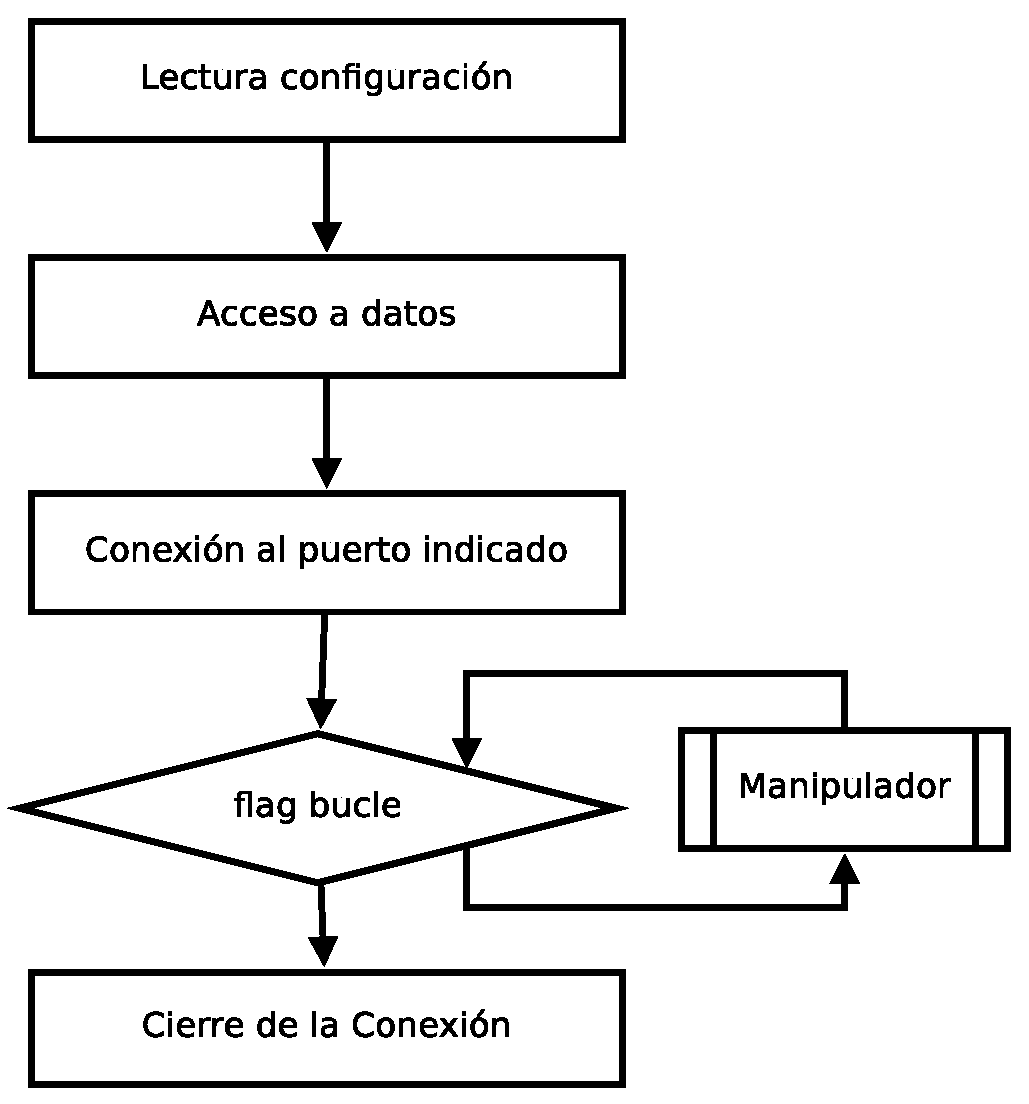
\includegraphics[width=0.45\textwidth]{img/FlujoServicio.eps}
              \caption{niveles OSI}
  \label{fig:nivelesOSI}
\end{wrapfigure}

En el contexto de los sistemas informáticos un protocolo es un conjunto de reglas predefinidas, cuyo proposito es estandarizar actividades y procesos. Siguiendo un mismo protocolo se garantiza que se mantendrá la compatibilidad entre los sistemas involucrados, independientemente del medio sobre el que est\'en en contacto, posiblemente otros protocolos.

La forma cl\'asica de programar un servicio consiste en un bucle de escucha que inicia subprocesos para cada conexi\'on entrante y que finaliza cuando esta acaba o se produce un error. Se presentan dos entidades en este caso, la del servicio que incluiria las rutinas para iniciar la escucha y el acceso a los datos y la del manipulador, que atiende la conexion siguiendo las pautas del protocolo.

\subsection{Servicio}

Al arrancar un servicio antes de iniciar el bucle de escucha deben realizarse una serie de procedimientos:
\begin{enumerate}
	\item La lectura de parámetros desde linea de comandos
	\item La lectura de parámetros desde el archivo de configuracion
	\item El registro de actividad en el(los archivo(s) pertinentes
	\item Preparar el acceso a los datos necesarios, ficheros o bases de datos
\end{enumerate}

\subsubsection{Parámetros}
Existen parametros que son comunes practicamente a cualquier servicio por ejemplo:
\begin{enumerate}
	\item Fichero de configuraci\'on.
	\item N\'umero de puerto para la escucha
	\item N\'umero m\'aximo de conexiones simultaneas
	\item Ficheros de registro, eventos, errores, etc
	\item Nivel de locuacidad (verbosity) en los registros.
\end{enumerate}
O parametros particulares para segun que tipos de servicio:
\begin{enumerate}
	\item Acceso al medio de datos
	\item Parametros de configuraci\'on concretos
\end{enumerate}
Debe tenerse en cuenta que los parametros en el fichero de configuracion tienen menor prevalencia que los indicados por linea de comandos, salvo el que especifique precisamente que fichero de configuracion debe leerse.

\subsubsection{Ficheros de configuración}
Debe acordarse una estructura común a todos los ficheros de configuración que se parsearán desde la plataforma pero permitiendo a la vez mantener la genericidad suficiente como para no perder la flexibilidad que haga este sistema util a cualquier implementacion de servicios y que a su vez permita que los usuarios puedan entender el fichero de forma clara y manipularlo facilmente.

Se espefican con ese fin las siguiente sintaxis:


\[<nombre parametro>=<valor>\{,<valor-N>\}\]


Para los valores que deben utilizar los parametros se pueden utilizar comodines para ampliar la versatilidad:
\begin{enumerate}
	\item \%H - Hostname
	\item \%i - Ip de la conexion entrante
	\item \%p - Puerto de origen de la conexion
	\item \%d - fecha actual
	\item \%t - hora actual
\end{enumerate}

\subsubsection{Locuacidad}
Para que puedan establecerse mensajes de depuración a distintos niveles debe adoptarse un sistema de categorias de mensajes, en cada etapa o proceso del servicio y del manipulador se emiten mensajes que incorporan el nivel de locuacidad para el que son generados, será la clase encargada de mostrar mensajes la que los muestre segun si el nivel de estos es menor o no que el indicado.
Se proponen los siguientes niveles
\begin{enumerate}
	\item 0 - Básico: mensajes de operaciones minimo, inicio del sistema, errores en los procedimientos.
	\item 1 - Moderado: mensajes comunes, entrada en servicio de un manipulador y puntos clave del desarrollo de la atención.
	\item 2 - Productivo: indica la entrada en la mayoria de las etapas de un servicio. Se amplian los detalles de los mensajes de error
	\item 3 - Expresivo: indica la entrada a cada etapa del servicio, se detalla el contexto de cada mensaje de error.
	\item 4 - Locuaz: detalla el contexto de cada etapa.
\end{enumerate}

\subsubsection{Registro}
Con la intencion de simplificar la tarea de gestionar la salida de mensajes, bien a la salida de la consola o a ficheros de registro deben implementarse clases destinadas a tal fin, que vuelquen o no los mensajes al medio según la locuacidad que se ha fijado y que en caso de que el medio predeterminado falle (por falta de espacio o cambio de permisos) sea capaz de cambiar a otro (indicado en la configuracion o a los medios salida por pantalla dedicados a tal fin).


\begin{figure}[h]
	\includegraphics[width=0.95\textwidth]{img/DiagramaClasesAnalisis.eps}
              \caption{Diagrama de Clases de Análisis}
     \label{fig:DiagramaClasesAnalisis}
\end{figure}


\subsection{Manipulador}
Precisamente es la naturaleza de un protocolo, como un conjunto ordenado de etapas en las que se organiza el flujo de informacion entre los sistemas, la que permite abstraer al programa servidor como un automata sensible al contexto. Cada etapa del manipulador equivale al estado del automata y pueden realizarse un conjunto determinado de acciones:
\begin{enumerate}
	\item Recibir datos desde la conexión
	\item Emitir datos a la conexión
	\item Tratar, almacenar o recuperar datos
	\item Avanzar, saltar o retroceder a otra etapa
\end{enumerate}

La recepción de los datos puede además controlarse mediante expresiones regulares según las especificaciones del protocolo, detectando rapidamente errores en la entrada. Debe facilitarse además la adopción de distintos tipos de intercambio de datos, controlados, formato en bruto o encriptados para evitar reimplementaciones de esta clase de rutinas.

En el diseño del manipulador debe tenerse en cuenta que normalmente existe un orden convencional en las etapas, previsiblemente estas deberia contener un numero limitado de procedimientos, para reducir la complejidad.

Durante la implementación de los protocolos ha aparecido la necesidad de trabajar sobre UDP. Para permitir esta funcionalidad y mantener un diseño eficiente se ha optado por dividir el manipulador en tres nuevas clases que permitieran trabajar tanto sobre el protocolo TCP como UDP y en concordancia a sus características:
\begin{enumerate}
	\item{Handler: la clase Handler primitiva se centra en la gestion de estados, el transito entre estos, y su inicializacion.}
	\item{TCPHandler: esta clase que hereda de Handler contiene una version especial de las rutinas de emision y recepcion de datos, se inicializa pasando el hash del socket.}
	\item{UDPHandler: Cada vez que un datagrama llega al servidor se instancia al manipulador, integrando la direccion de origen del datagrama y los datos que portaba, esta clase tendra sus propias rutinas de emisión y recepción. Debe tenerse en cuenta que en este tipo de manipulador se hace necesario algun sistema que permita recuperar desde el servidor en que estado se encontraba al finalizar la última transmision.}
\end{enumerate}
\subsection{Flujos de los protocolos}
A continuación se va a espeficicar el flujo de los protocolos con los que se va a probar la plataforma.

\subsubsection{Telnet}
\begin{figure}[h]
	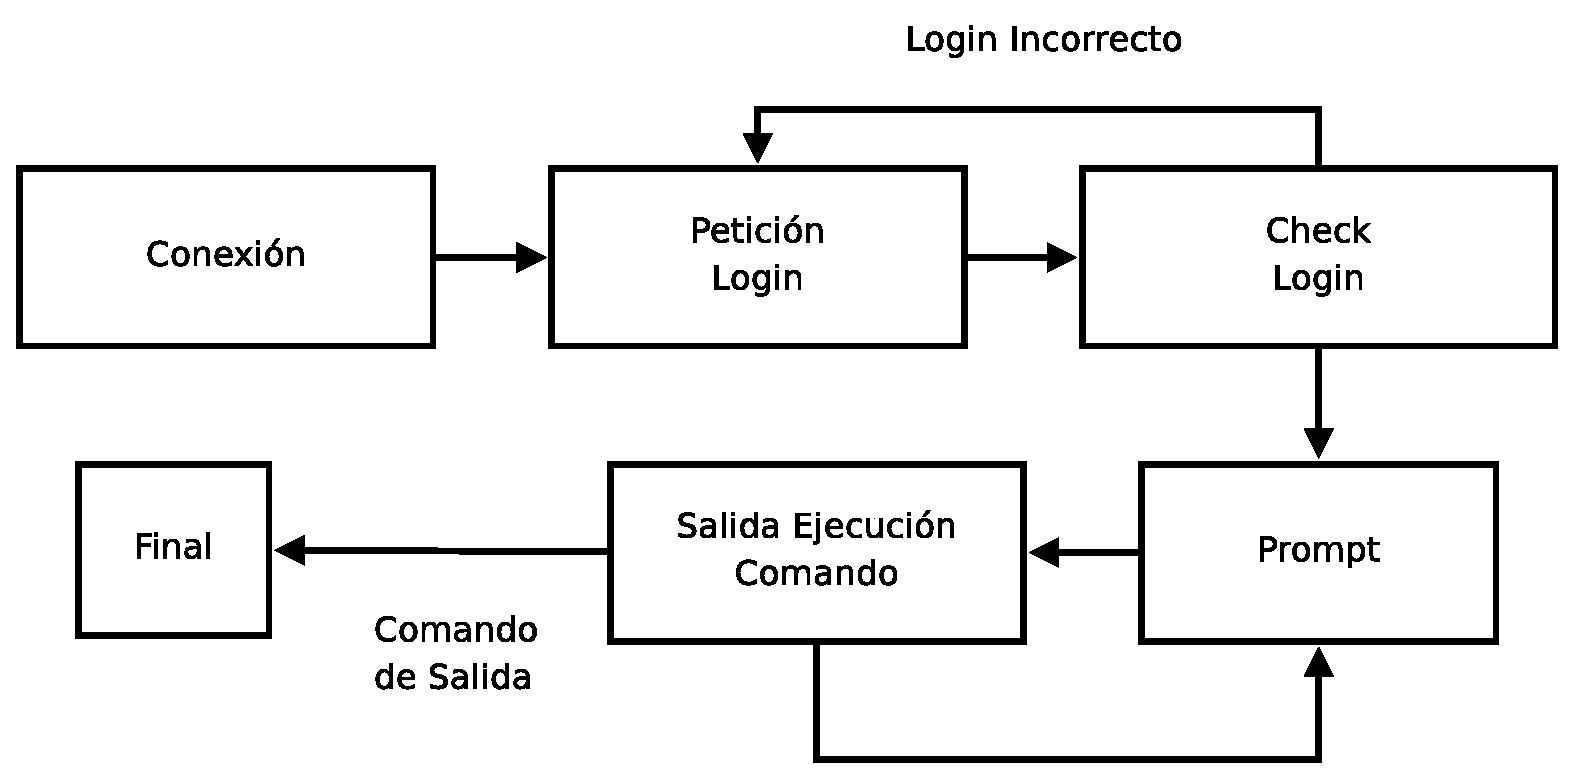
\includegraphics[width=0.95\textwidth]{img/DiagramaFlujoTelnet.eps}
              \caption{Flujo de desarrollo del protocolo Telnet}
  \label{fig:DiagramaFlujoTelnet}
\end{figure}

El protocolo Telnet tiene un flujo básico de desarrollo muy simple:
\begin{enumerate}
	\item Se establece la conexión con el cliente
	\item Se presenta el dialogo de peticion de contraseña y se espera a que se introduzcan los datos.
	\item Se checkea la contraseña contra la base de datos correspondiente
	\item Se solicita el comando a ejecutar en el sistema
	\item Se ejecuta el comando pertinente y se muestra su salida. y se vuelve al paso 4.
\end{enumerate}
Existe un pequeño conjunto de pasos alternativos:
\begin{enumerate}
	\item (4.Alternativo) El usuario debe repetir la autentificación
	\item (5.Alternativo) Se ha solicitado finalizar la sesión con lo que procedemos a la desconexión.
\end{enumerate}
\subsubsection{HyperText Transfer Protocol}
\begin{figure}[h]
	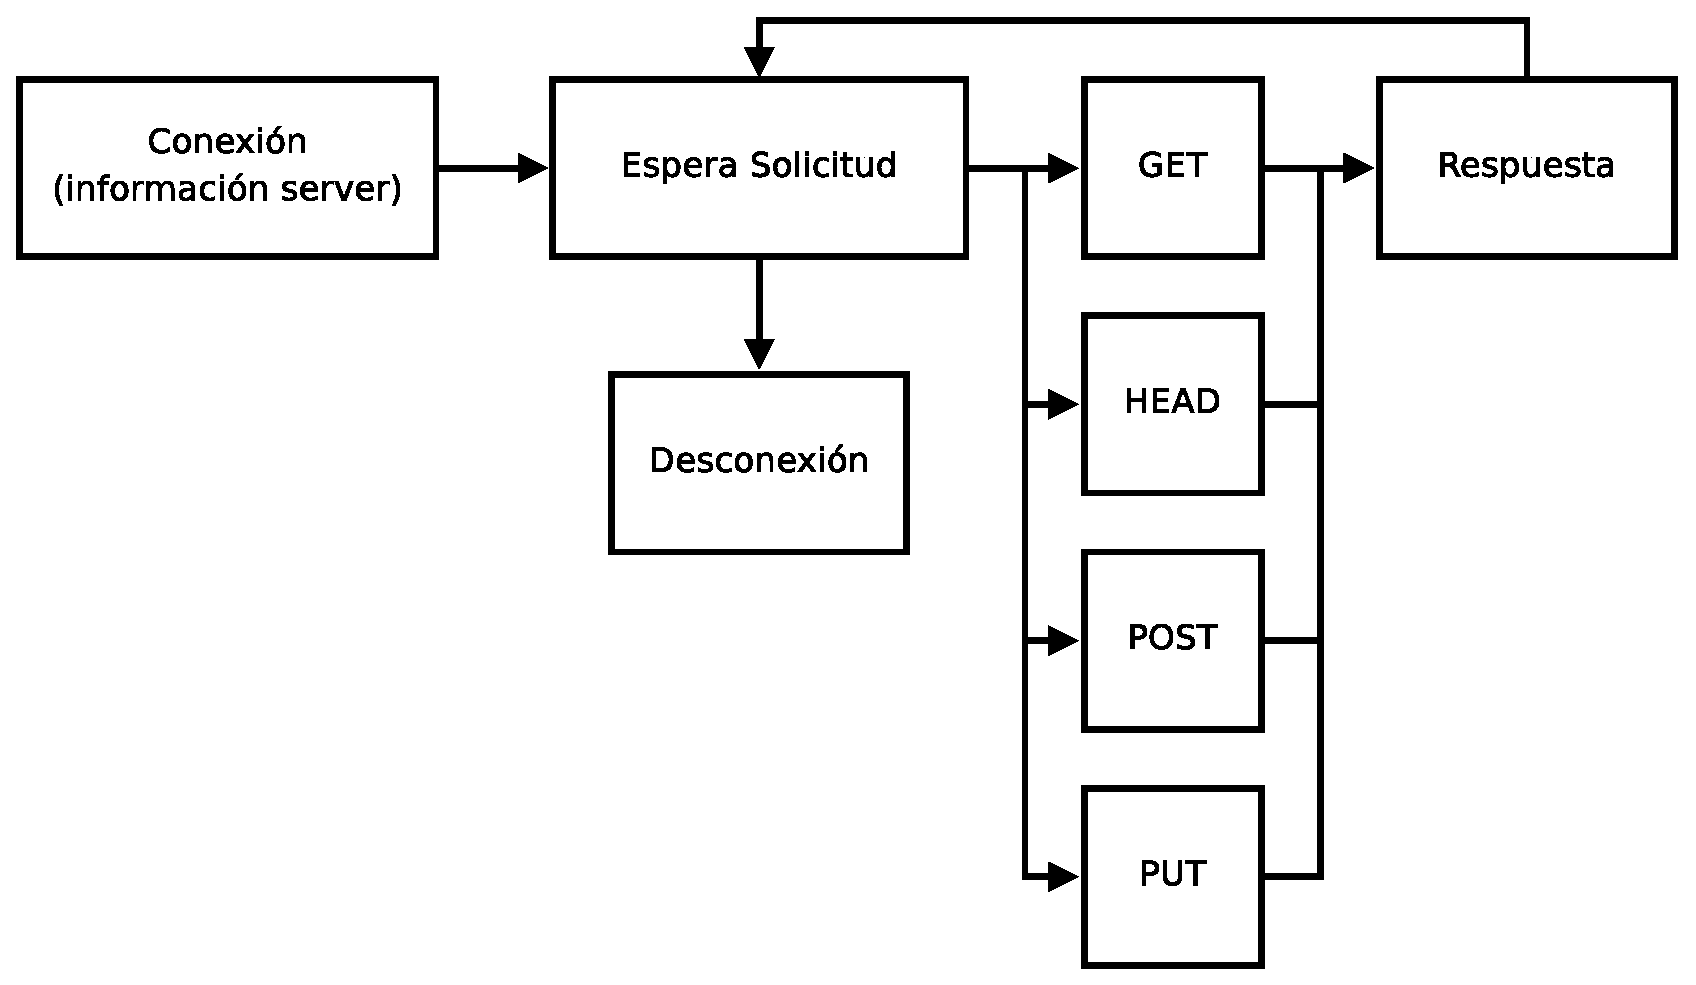
\includegraphics[width=0.95\textwidth]{img/DiagramaFlujoHTTP.eps}
              \caption{Flujo de desarrollo del protocolo HTTP}
  \label{fig:DiagramaFlujoHTTP}
\end{figure}
El protocolo HTTP/1.1 tiene un flujo basico bastante más amplio, ya que despues de recibir la orden las rutinas que atenderán el comando difieren drasticamente, en consecuencia deberán implementarse nuevos estados para cada tipo de comando.
\begin{enumerate}
	\item Se establece la conexión con el cliente
	\item Se muestra la información del servidor
	\item Se reciben las cabeceras y el comando
	\item En el estado de atencion se recibe el resto de la información (si procede)
	\item Se responde informando del estado.
\end{enumerate}
Aunque la conexión pueda perderse inesperadamente en cualquier momento, es en el momento de esperar el comando cuando se produciría una desconexión correcta.
\subsubsection{Session Initialization Protocol}
El protocolo SIP es responsable de varias tareas, aunque puede operar sobre UDP la implementación sobre BLAS solo funcionará sobre UDP. Estas tareas son:
Es precisamente en este punto por la necesidad de trabajar sobre UDP cuando se ha tomado la decisión de dividir el manipulador en tres nuevas clases que permitieran trabajar tanto sobre el protocolo TCP como UDP y en concordancia a sus características.
\begin{figure}[h]
	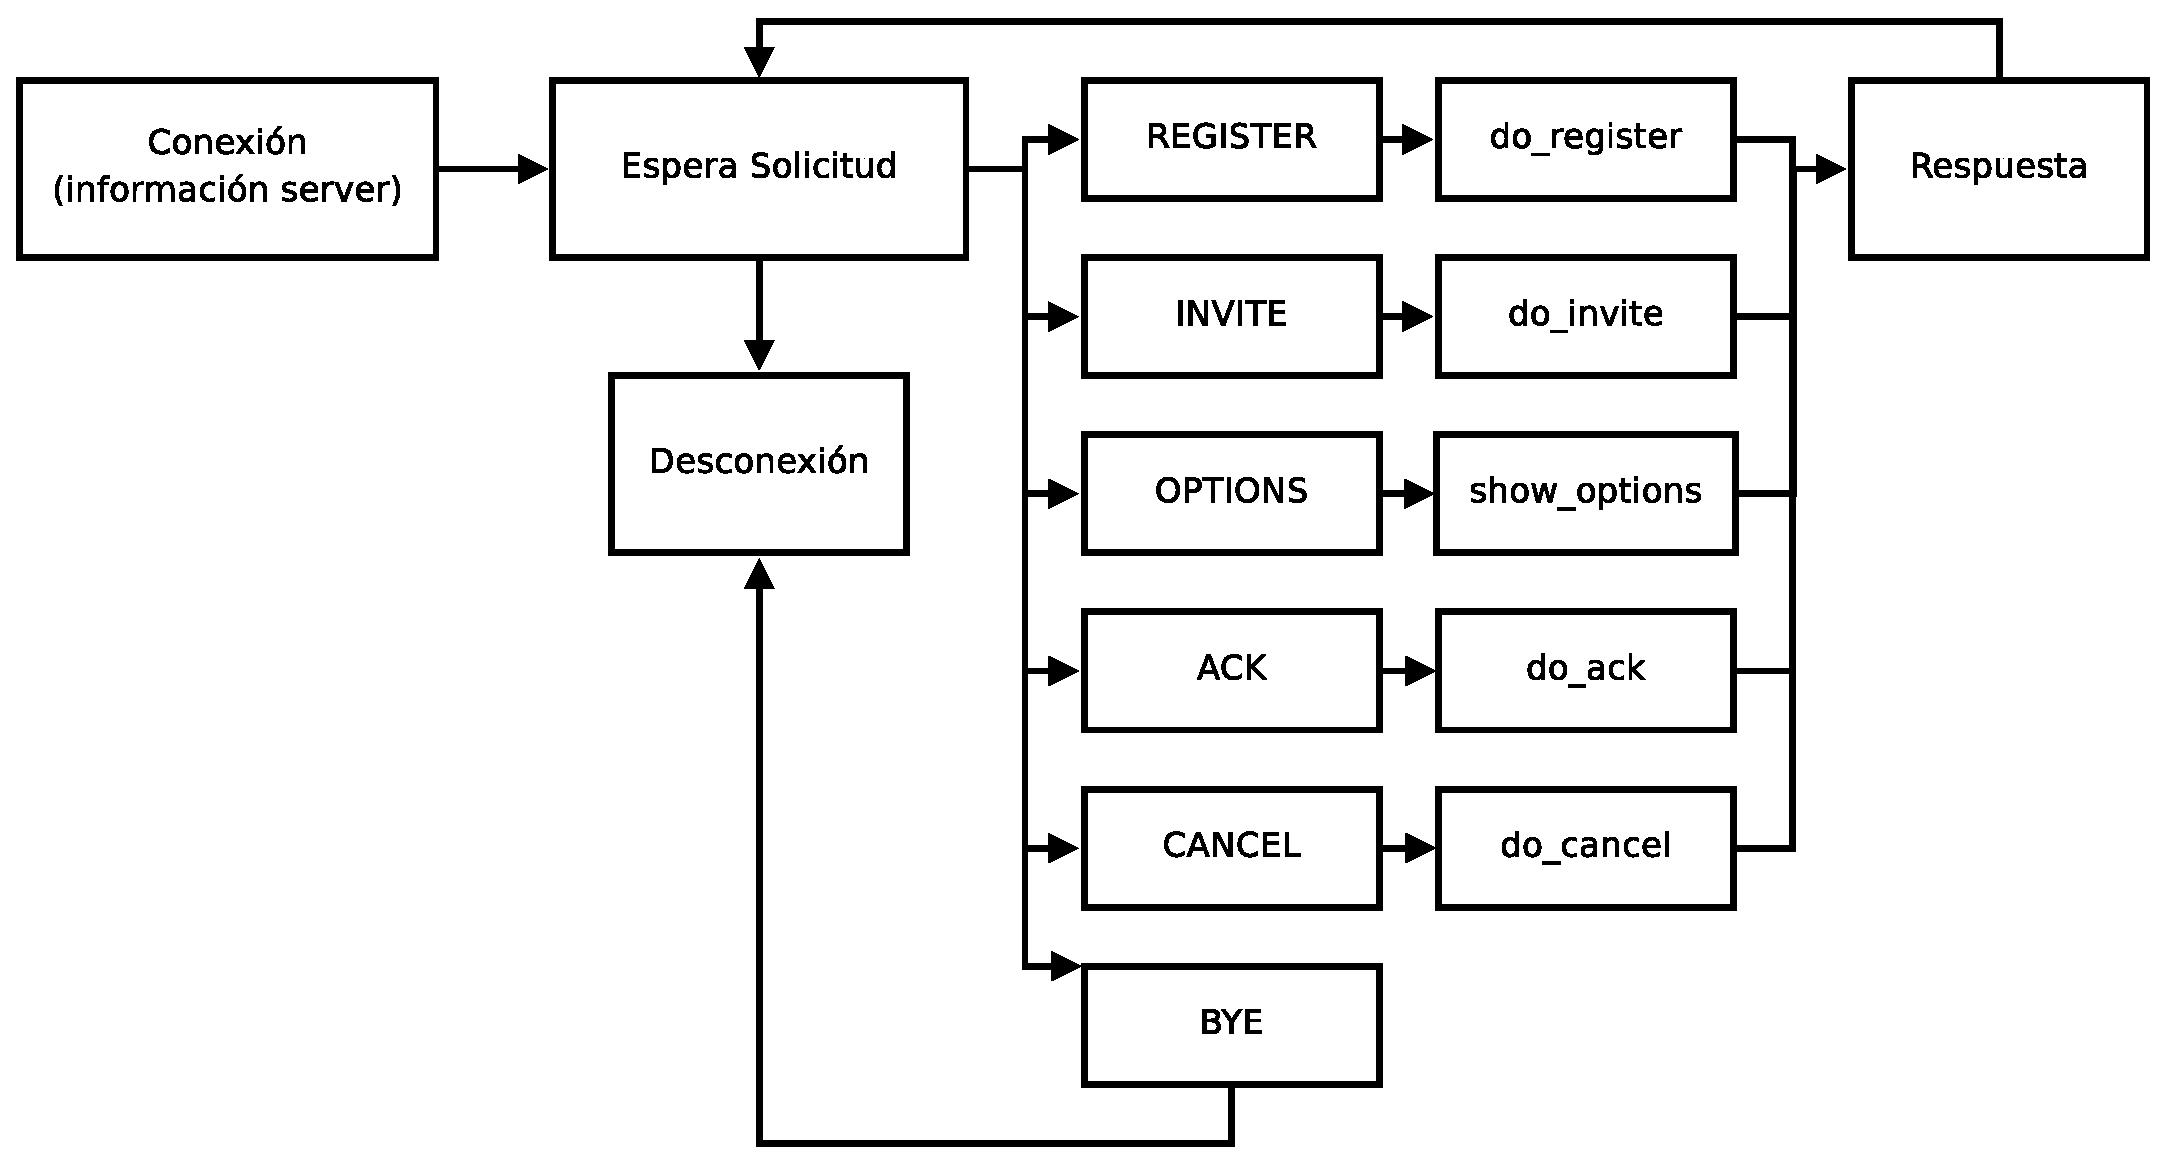
\includegraphics[width=0.95\textwidth]{img/DiagramaFlujoSIP.eps}
              \caption{Flujo de desarrollo del protocolo SIP}
  \label{fig:DiagramaFlujoSIP}

\end{figure}

\begin{enumerate}
	\item{Registro(REGISTER): El usuario se da de alta en el sistema y figura en el directorio de usuario.}
	\item{Invitación(INVITE): Dirigido a un usuario se le autoriza a acceder a un medio compartido. Debe aceptarse con ACK o denegarse con CANCEL.}
	\item{Opciones(OPTIONS): Solicita al servidor el listado de las funcionalidades.}
	\item{Cierre(BYE): Avisa de que va a procederse con la desconexión.}
\end{enumerate}


\subsection{Acceso a datos}
Muchos servicios tienen la necesidad de leer y escribir en medios de datos centralizados, por eso es importante diseñar según se debe hacer un esfuerzo en desarrollar un modelo de acceso a datos que permita una lectura lo más transparente posible, facilitando la lectura del codigo. 

Normalmente existen unos tipos limitados de medios de datos:
\begin{enumerate}
	\item{Registos unificados volátiles: Son medios de datos que se borrarán cuando se desactive el servicio, deben permitir el acceso concurrente por parte de los hilos. Este tipo de medios sería muy adecuado para sistemas de chat etc.}
	\item{Accesos a bases de datos: Python tiene soporte para acceder a muchos tipos de bases de datos: Mysql, Postgresql, ODBC, etc. Sin embargo diseñar un acceso a datos mediante objetos que eviten la manipulacion de peticiones SQL en el codigo de la atención del servicio será básico para la comprensión del codigo y su depuración}
	\item{Acceso remoto a datos: En ocasiones los datos que se necesitan estarán en sistemas remotos, accediendo a ellos mediante conexiones IP/TCP y normalmente sobre estos metodos HTTP, SOAP o REST. Al igual que en otros medios de acceso es importante que el metodo de acceso se abstraiga del codigo de atención del servicio}
\end{enumerate}
En definitiva y aunque para cada tipo de servicio el modelo de acceso a datos varía considerablemente se pueden establecer las siguientes lineas para el analisis y la orientación que tomará el sistema:
\begin{enumerate}
	\item{Claridad: Debe evitarse la molesta aparición de lineas SQL, peticiones HTTP, XML y similares en el codigo.}
	\item{Orientación a objetos: Un buen modelo de acceso a datos reducirá sensiblemente el tiempo que se requiera para depuración y posteriores.}
	\item{Manejo de errores: Es importante integrar el manejo de excepciones en las rutinas de adquisición de datos ya que no estarán exentas de fallos.}
	\item{Oportunidad de acceso: Deben elegirse adecuadamente en que momentos se accederá a los datos, para no producir latencias en puntos del proceso sensibles al tiempo de respuesto.}
\end{enumerate}

\section{Diseño}

\subsection{Librería principal}
Existe una parte común a toda la plataforma que contiene las clases abstractas:

\begin{figure}[h]
	\includegraphics[width=0.80\textwidth]{img/DiagramaClasesDisennoCore.eps}
	\caption{Diagrama de Clases de la librería principal} 
	      \label{fig:DiagramaClasesDiseñoCore}
\end{figure}

En estas clases se incorporarán todas las funcionalidades que puedan emplearse desde cualquier implementación de un servicio. Para simplificar el procedimiento de herencia de componentes se incluiran todas en el archivo core.py, que acompañaría al archivo que contenga el código del servicio en si mismo en cada despliegue que se haga a posteriori del sistema.
\subsubsection{Server}
Esta clase incluye las rutinas necesarias para la inicializacion y configuración del servicio:
\begin{enumerate}
	\item Carga y parseado de los parámetros de linea de comando.
	\item Carga e interpresatcion de los archivos de configuración.
	\item Reserva del socket al que se conectarán los clientes del servicio.
	\item Bucle principal de inicializacion y despacho de los hilos.	
	\item Inicialización de los registros de eventos y errores del sistema.
	\item Recopilación de las cadenas de documentación relacionadas con cada parametro del sistema.
	\item Inicialización de los medios de acceso a datos comunes (si procede). 
\end{enumerate}
\subsubsection{Error}
Esta clase que hereda de la clase de sistema Exception se utiliza como tipo de datos por defecto en caso de que alguno de los procesos o rutinas del sistema no pueda realizar su función, en estos casos devolverá un objeto de clase Error.

Además Error contiene 2 datos importantes para la infraestructura:
\begin{enumerate}
	\item msg:string contiene una cadena explicando el suceso que originó el error.
	\item level:integer se utiliza para saber si la gravedad del suceso obliga a su aparición en los registros.
\end{enumerate}
Los metodos son una sobrecarga de los metodos basicos de la clase Exception:
\begin{enumerate}
	\item \_\_init\_\_ Que inicializa el objeto proveyendo de la información con el mensaje de error y el nivel de importancia.
	\item \_\_str\_\_ Devolverá la cadena con la explicación del error y el nivel de importancia cuando se necesite imprimirlo en el registro.
\end{enumerate}
\subsubsection{Log}
En esta versión del registro solo se volcarán los eventos y errores a salida estandar o a ficheros. Para reducir el acoplamiento en las llamadas en los objetos de registro integran los siguientes datos durante su tiempo de vida:
\begin{enumerate}
	\item file:File salvo que su valor sea None será el descriptor de fichero donde se volcará la información.
	\item level: Int indicará el nivel de importacia que debe igualarse o superarse para que el evento se vuelque en el registro.
\end{enumerate}
Los m\'etodos propios de los objetos tipo Log son:
\begin{enumerate}
	\item \_\_init\_\_() m\'etodo de inicialización del registro, indicando el nombre del fichero de volcado y el nivel mínimo de importancia. Si la apertura del fichero falla se pasarán a volcar los datos a la salida estandar.
	\item put() con este m\'etodo se vuelcan eventos al registro, además del mensaje debe acompañarse del nivel de importancia del evento. Para simplificar su invocación normalmente se utiliza un puntero desde self.log[``report''].put() a self.report() con lo que las llamadas son mucho más cortas.
\end{enumerate}
\subsubsection{Handler: UDP y TCP}
Seguramente las clases más importantes que se incorporan en un servicio:
\begin{enumerate}
	\item Handler: Es la clase principal, hereda de la clase hilo (Thread) y sus principales funcionalidades son:
		\begin{enumerate}
			\item Cnotrolar el avance, retroceso y transito entre estados del manipulador en ejecución.
			\item Sobrecargar las clases minimas de la clase Thread para un funcionamiento coherente.
		\end{enumerate}
	\item TCPHandler: Versión del manipulador que contiene los atributos y m\'etodos concretos para tratar con el socket que les corresponda, en este caso basta con guardar el puntero al Socket, ya que es lo unico que necesitan las rutinas send() y receive() para enviar y recibir datos con el cliente.
	\item UDPHandler: Versión del manipulador destinada a atender las peticiones UDP. En el caso de protocolo UDP es más complicado ya que no existe un Socket como tal, en su lugar se guardar la ip y puerto de donde procedía la comucación y ademas el buffer de los datos recibidos. Con lo que los procedmientos de envio y recepción de datos tienen las siguientes particularidades:
		\begin{enumerate}
			\item send(): debe crear un nuevo socket UDP con los datos de conexión que posee, estos pueden facilitarse desde los parámetros o utilizar los que figuran como origen de los datos. No existe confirmación sobre si los datos han llegado por lo que la aplicación debe buscar su forma de confirmar la transmisión.
			\item receive(): Todos los datos que puedan llegar al hilo de atención llegan de una sola vez desde el momento en que se inicia, se van consumiendo según especifique el patrón que se pasa como parámetro. Si el buffer de datos está vacio se devolvera un Error.
		\end{enumerate}
\end{enumerate}
\subsection{Servicio de ejemplo}
A continuación se presenta un ejemplo de como se realiza la implementación de un servicio heredando de las clases de BLAS.

\begin{figure}[h]
	\includegraphics[width=0.80\textwidth]{img/DiagramaClasesDisennoParticular.eps}
	\caption{Diagrama de Clases de un servicio de ejemplo} 
	      \label{fig:DiagramaClasesDiseñoParticular}
\end{figure}
El arranque del sistema se realiza de la siguiente manera:
\begin{enumerate}
	\item Se carga el fichero con el interprete de python, presumiblemente el fichero se llamaría particular.py.
	\item Una vez finalizadas las importaciones de los modulos se cargan las definiciones de clases y sus m\'etodos.
	\item Cuando se llega a la zona de ejecución se instancia un objeto ParticularServer con los argumentos recibidos por linea de comandos, despu\'es se invoca al m\'etodo mainloop indicandole la clase de manipulador que debe instanciar.
	\item Durante la inicializacion de un objeto ParticularServer se instancian a su vez los objetos de registro, a su vez se llama a la inicializacion de Server, que será común a todos los servidores, aqui se parsearán las opciones de la linea de comandos, cuyas directrices estarán distribuidas en el codigo de ParticularServer y Server en m\'etodos que inician su nombre con ``config\_'' seguido del nombre del parámetro, en su campo de documentación se incluye el prefijo que debe utilizarse en la linea de comandos para modificar estos parámetros.
	\item En mainloop() discriminando el tipo de manipulador(TCP o UDP) abrirá el tipo de socket pertinente e iniciará un bucle while. Dentro de estelas conexiones se irán atendiendo por parte de los manipuladores. Para que los manipuladores puedan hacer su trabajo deben primero inicializarse y luego emitir la orden de arranque.
	\item Al inicializar el hilo del manipulador se le aporta bien el socket de conexión para los tipo TCP y el buffer y la dirección de origen para los UDP. El m\'etodo start() que se hereda de la clase Thread iniciará la ejecución del hilo que se desarrollará a lo largo de los estados que se deban seguir para atender la petición.
	\item la mayor parte del codigo del manipulador serán m\'etodos cuyo nombre empiece port ``step\_'' seguido del identificador del paso en si mismo, en cada paso debe indicarse si se pasa al siguiente, al anterior o se salta a otro, de otra manera se repetirá el mismo paso.
\end{enumerate}
\chapter{Previsiones y proyectos futuros}
\section{Mejoras}
En futuras implementaciones de BLAS se preveen una serie de mejoras planteadas para aumentar la funcionalidad de la plataforma o solventar sus carencias

\subsection{Cifrado}
Actualmente casi todos los servicios de red se comunican empleando canales seguros. Probablemente imitar cualquier servicio de forma completa requeriría aportar el soporte de distintos metodos criptograficos. Algunos de los algoritmos mas comunes que se pueden localizar en internet son:
\begin{enumerate}
	\item{DES y 3DES: Publicados en 1976 y 1978 respectivamente son los algoritmos más veteranos y aun presentes en muchos sistemas aunque hayan perdido robusted con el paso del tiempo.}
	\item{IDEA: Publicado en 1991 para sustituir a DES}
	\item{Blowfish: Publicado en 1993}
	\item{RC5: Publicado por RSA en 1994}
\end{enumerate}
Para facilitar su uso por parte del programador y así mantener uno de los principales valores de la plataforma deben diseñarse metodos para que una vez negociada una contraseña común el flujo de datos pueda mantenerse de forma identica al uso que se realizara sobre send() y receive(). Ya que python permite la sobrecarga de metodos desde la propia clase durante la ejecución implementar una rutina que reemplace los metodos de entrada y salida no revestirá dificultad.

\subsection{Sistemas de registro opcionales}
Además del volcado de la información de registros de operación y errores al sistema de ficheros o a la salida estandar, existen otras posibilidades que pueden extender la funcionalidad de la plataforma:
\begin{figure}[h] %{h}{0.65\textwidth}
	%{figure}[h]
	\includegraphics[width=0.65\textwidth]{img/DiagramaClasesDisennoNewLogs.eps}	
              \caption{Diagrama de diseño nuevos registros}
  \label{fig:DiagramaClasesDisennoNewLog}
\end{figure}

\begin{enumerate}
	\item{Terminal TCP: Consistente en un servicio que tras conectarse mediante telnet permita revisar los eventos en el sistema.}
	\item{Volcado UDP: se enviarán a una ip y puerto predeterminados la información en texto claro de los eventos del sistema.}
\end{enumerate}

De esta manera se debería extender la clase Log, creando nuevas subclases que heredarian de Log, sobrecargando los metodos para actuar de forma transparente al programador.


\subsection{Establecimiento como servicio del sistema}
Ya que python es multiplataforma según BLAS madure deberían acompañarsele procedimientos faciles para que los servicios producidos puedan implantarse en el sistema junto a otros.

Es importante implementar una rutina que permita un empaquetado facil del codigo y el software asociado (el imterprete Python con el juego de librerias necesario) para un despliegue del sistema lo mas agil y rápido posible.

\subsection{Construcción de expresiones regulares}
La construcción de expresiones regulares que acepten cadenas de acuerdo a un patron consumen tiempo y en ocasiones son el origen de fallos dificiles de diagnosticar. Por este motivo implementar un sistema para construir expresiones regulares de forma rapida y clara debería ser una de las prioridades a la hora de extender el proyecto.

El resultado ideal sería conseguir que no aparezcan expresiones regulares que entorpezcan la lectura del codigo de atención del servicio.
\section{Rendimiento y pruebas}
Para profundizar en las capacidades de la plataforma para implementar servicios en cierto nivel de producción deberían realizarse una serie de estudios
\subsection{Benchmarking}
Comparando con el rendimiento de otros servicios implementados sobre lenguajes mas ligeros como C debería ofrecer una idea de que necesidad de recursos tiene la plataforma en funcion de la cantidad de clientes y el tipo de exigencia de estos. Conociendo estos requisitos podrán conocerse las posibilidades reales de que el prototipo pueda entrar en algún nivel de producción.

Sería interesante realizar distintos intentos según el nivel de optimización con que se configure la compilación a bytecode del producto.


\subsection{Seguridad}
Para obtener datos fiables sobre la confiabilidad del servicio producido, sobretodo si está expuesto a accesos de terceros, deben realizarse pruebas con intención de desestabilizar el programa o incluso acceder a recursos restringidos a traves de el.


\end{document}

